\documentclass[lettersize,journal]{IEEEtran}
\usepackage{amsmath,amsfonts}
\usepackage{algorithmic}
\usepackage{array}
\usepackage[caption=false,font=normalsize,labelfont=sf,textfont=sf]{subfig}
\usepackage{textcomp}
\usepackage{stfloats}
\usepackage{url}
\usepackage{verbatim}
\usepackage{graphicx}
\usepackage{cite}
\usepackage{balance}
\usepackage[acronym]{glossaries}
\usepackage{cleveref}
\usepackage{subcaption}

\makeglossaries

% Define acronyms
\newacronym{adam}{ADAM}{Adaptive Moment Estimation}

\begin{document}

% EXAMPLES

% \begin{figure*}[h]
%   \centering
%   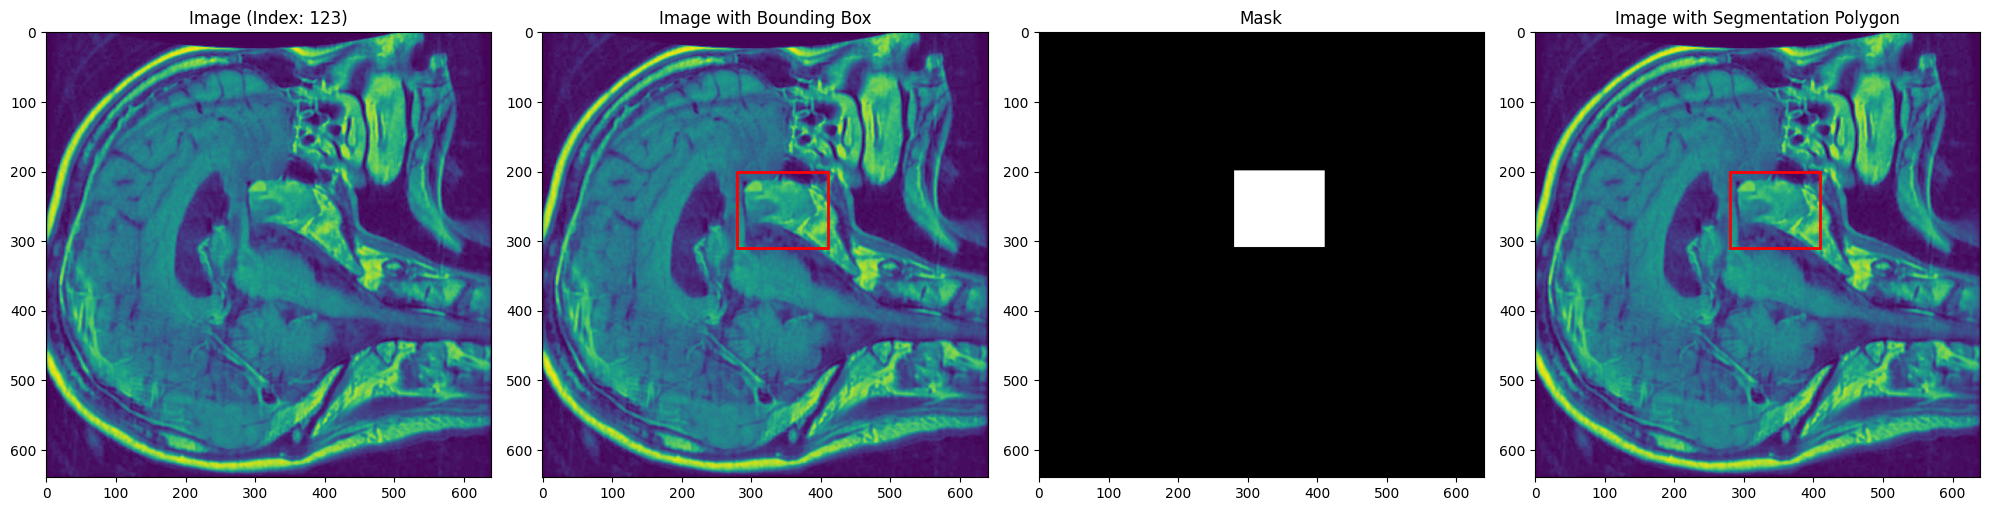
\includegraphics[width=\textwidth]{images/du_image_and_mask.png}
%   \caption{Plot of a sample image from the data set, the image with bounding box, the corresponding mask and the visualization of the polygon to show that the polygon does not contain any further useful information compared to the bounding box.}
%   \label{fig:da_image_and_mask}
% \end{figure*}

% \begin{figure*}[h]
%   \centering
%   \subfloat{\label{fig:image5}%
%       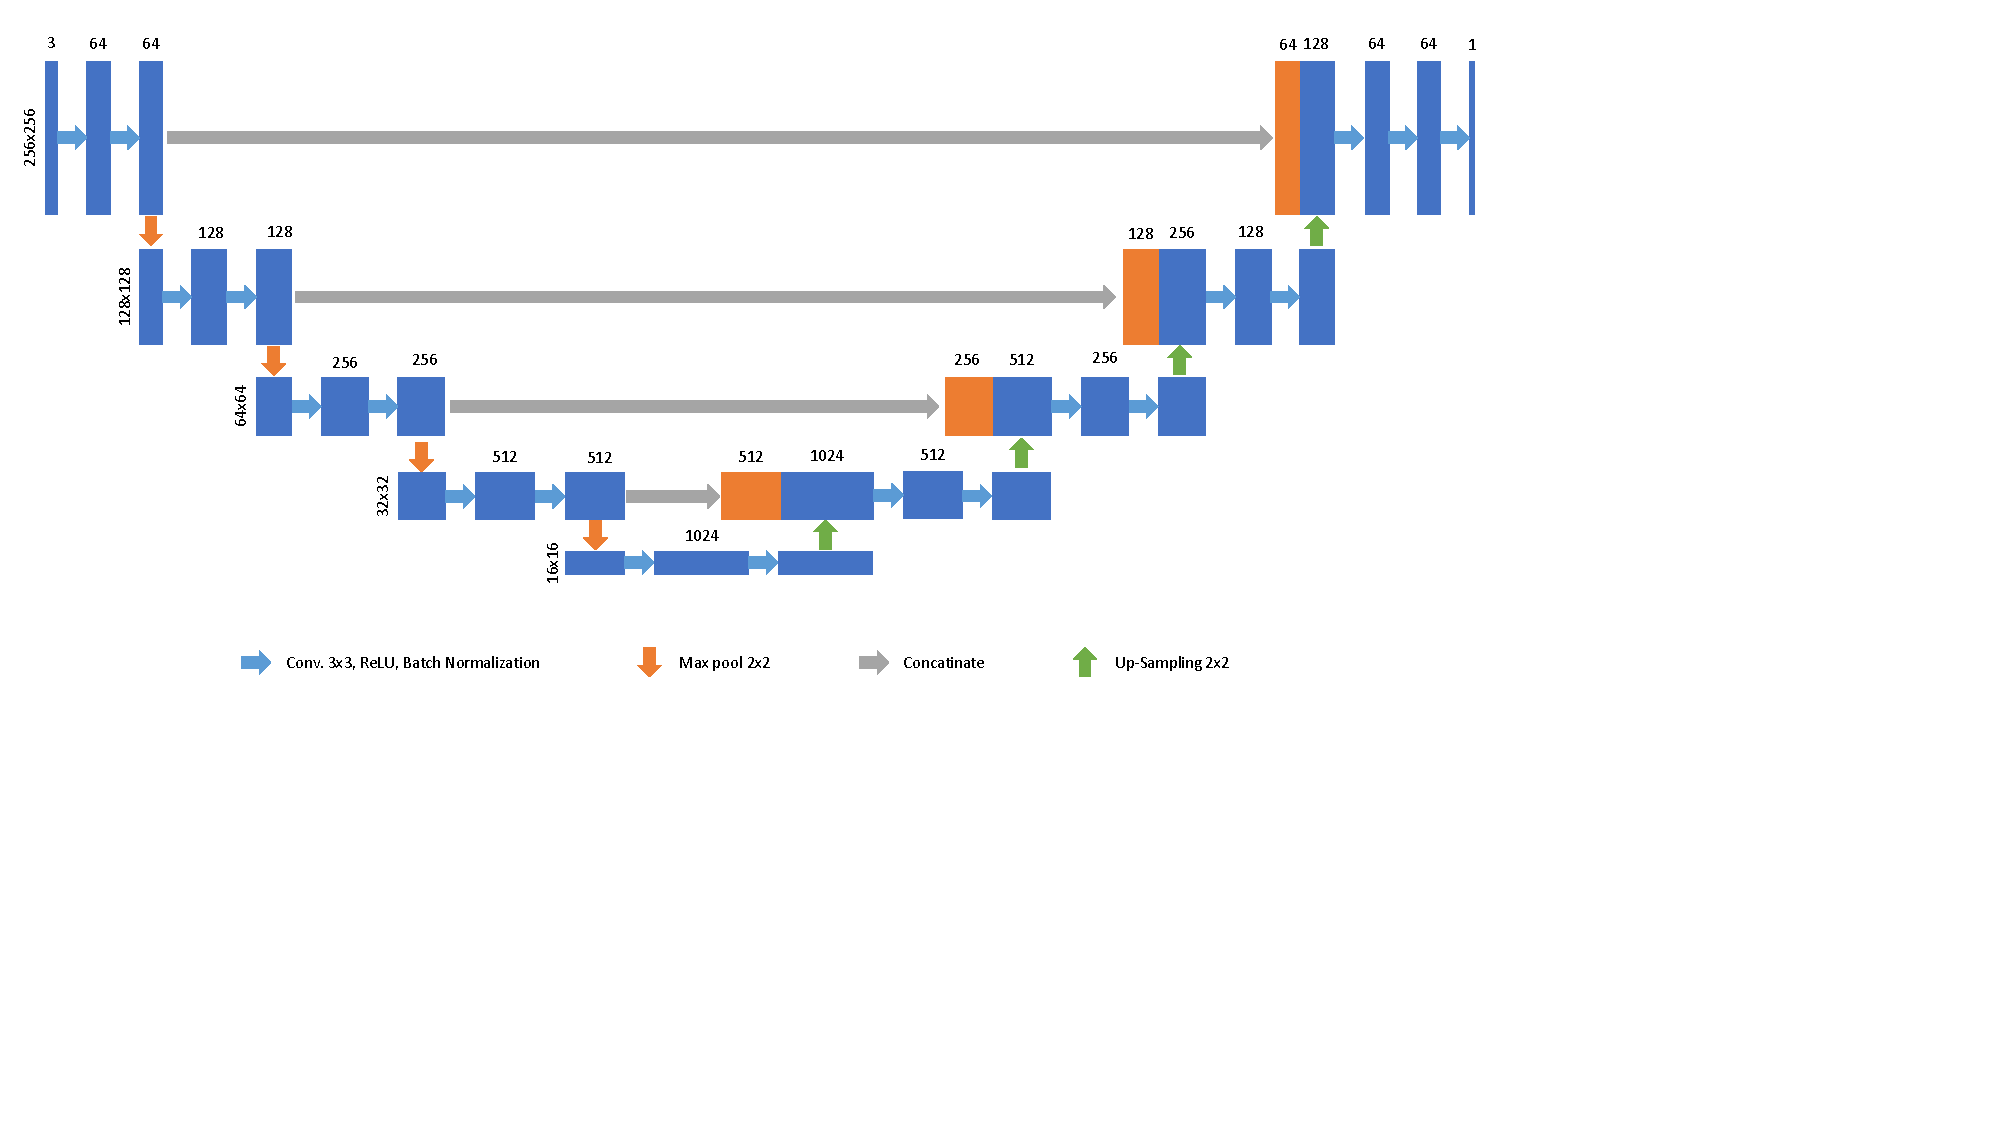
\includegraphics[width=0.45\textwidth]{images/Selfdesigned_unet.pdf}} \quad
%   \subfloat{\label{fig:image6}%
%       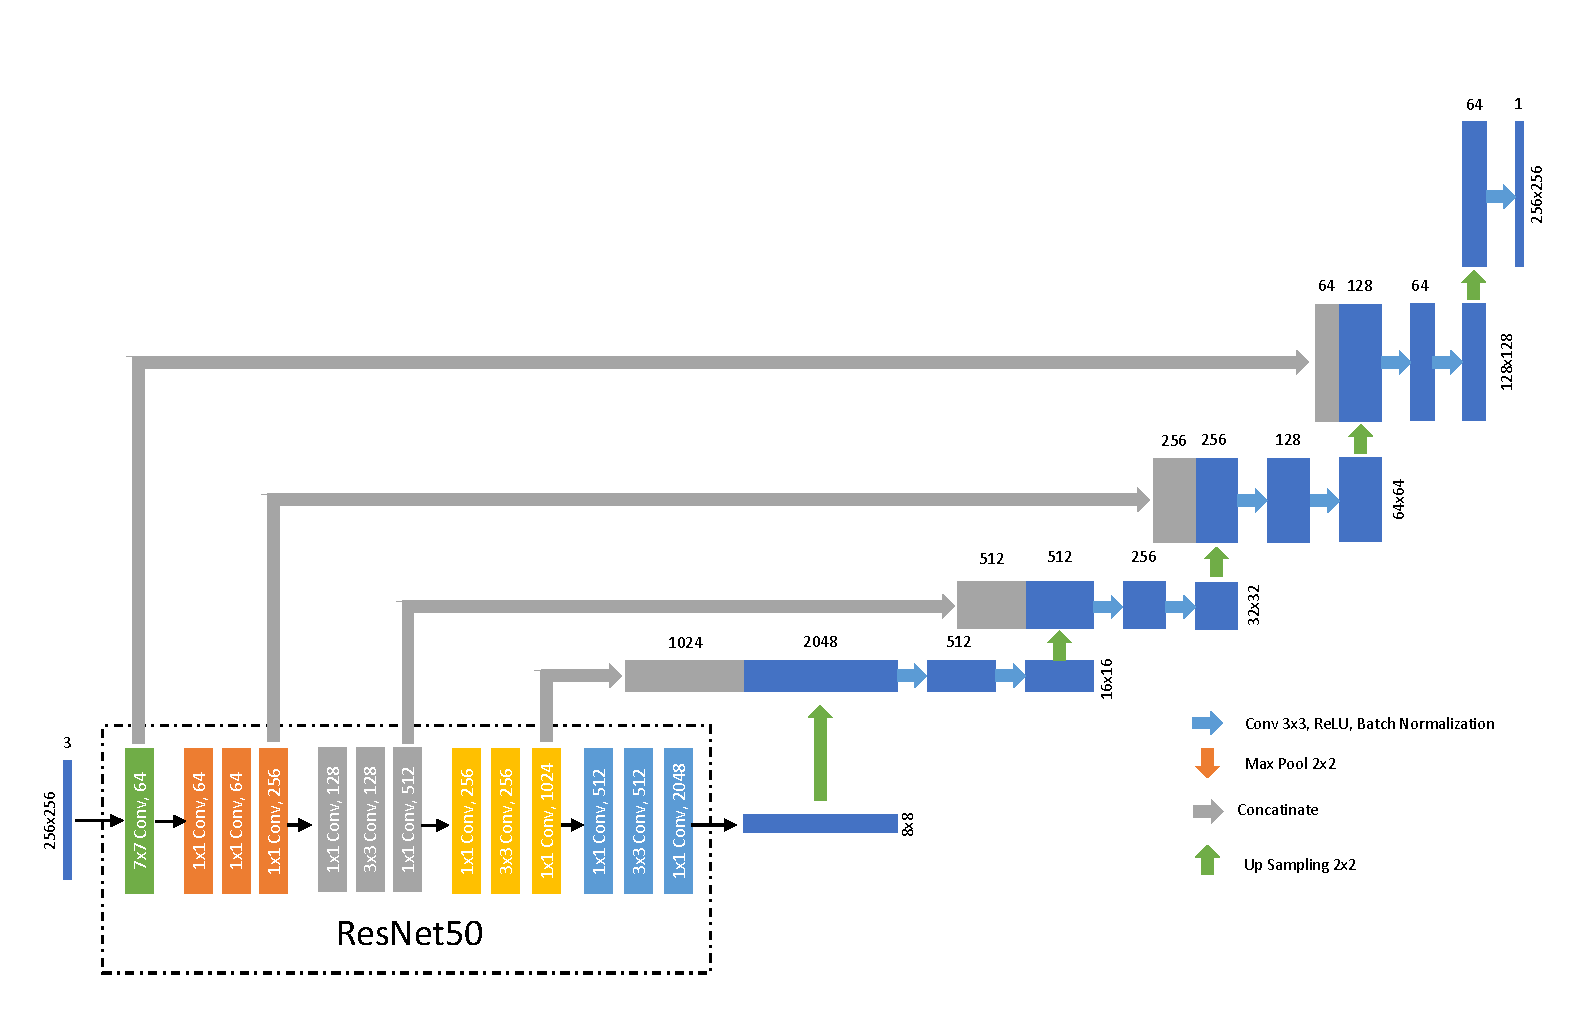
\includegraphics[width=0.45\textwidth]{images/Pretrained_unet-cropped.pdf}}
%   \caption{Model architectures of the self-designed UNet and the UNet with pre-trained ResNet50 backbone}
%   \label{fig:models}
% \end{figure*}

% Acronym \gls{adam} 
% Formula terms \( y \) and \( \hat{y} \). Equation:

% \begin{equation}
% {L} = - \left( y \log(\hat{y}) + (1 - y) \log(1 - \hat{y}) \right)
% \end{equation}

% In alignment to the definitions above we used the following formulas to calculate the evaluation metrics of our models with \( y_i \) and \( \hat{y}_i \) representing the actual and predicted values for the \(i\)-th pixel, respectively, and the total number of pixels denoted by \( N \):
% \begin{itemize}
%   \item \textbf{Accuracy} is the ratio of correctly predicted pixels to the total number of pixels:
%   \begin{equation}
%   \text{Accuracy} = \frac{1}{N} \sum_{i=1}^{N} \left( y_i \hat{y}_i + (1 - y_i) (1 - \hat{y}_i) \right)
%   \end{equation}
% \end{itemize}


\title{Title}

\author{Jakob Müller
\thanks{This work is created as a student research project at the Cooperative State University Baden-Württemberg Center for Advanced Studies at Heilbronn. The opinions expressed here are entirely that of the author. No warranty is expressed or implied. User assumes all risk.}}
\markboth{DHBW Center for Advanced Studies, Prof. Dr. Dirk Reichardt, July~2024}%
{Title}



\maketitle



\begin{abstract}
  Abstract.
\end{abstract}



\begin{IEEEkeywords}
Keyword, Keyword.
\end{IEEEkeywords}


\section{Introduction}
\IEEEPARstart{R}{elevance}, Challenge, Objective, Goal, Research Question/Answer, Hypotheses


\section{Related Work}



\section[Methods]{Dataset}



\section[Methods]{Methods}
%( Method, Approach** (incl. theory), Development method (data, model architecture, hyperparameters, ...) )

\section[Results]{Results}


\section{Conclusion}


\balance

\bibliographystyle{IEEEtran}
\bibliography{bib_CV_MRI_ImSeg}

% \begin{thebibliography}{1} %Example of a Citation: According to a well-known study \cite{ams}, the mathematical typesetting is crucial for clear presentation.

% \bibitem{ams}
% {\it{Mathematics into Type}}, American Mathematical Society. Online available: 

% \bibitem{oxford}
% T.W. Chaundy, P.R. Barrett and C. Batey, {\it{The Printing of Mathematics}}, Oxford University Press. London, 1954.

% \bibitem{lacomp}{\it{The \LaTeX Companion}}, by F. Mittelbach and M. Goossens

% \end{thebibliography}


\end{document}

